%% IEEE Access journal submission
%% Class: IEEEtran v1.8b (https://www.ctan.org/pkg/ieeetran)
%% Compile: pdflatex main.tex && bibtex main && pdflatex main.tex && pdflatex main.tex
%%          (or: latexmk -pdf main.tex)

\documentclass[journal,onecolumn,11pt]{IEEEtran}

\usepackage[T1]{fontenc}
\usepackage[utf8]{inputenc}
\usepackage{lmodern}
\usepackage{microtype}
\usepackage{amsmath,amssymb,amsfonts}
\usepackage{booktabs}
\usepackage{multirow}
\usepackage{array}
\usepackage{xcolor}
\usepackage{graphicx}
\usepackage{url}
\usepackage{hyperref}
\usepackage{cite}
\usepackage{tikz}
\usepackage{tcolorbox}
\usepackage{textcomp}

\hypersetup{colorlinks=true, linkcolor=blue!60!black, citecolor=blue!50!black,
            urlcolor=blue!60!black, pdfauthor={Vu Dang},
            pdftitle={Beyond English-Only GRPO}}

\setlength{\emergencystretch}{3em}
\hyphenpenalty=1000
\sloppy

\renewcommand{\UrlBreaks}{\do\/\do-\do_\do.\do=\do?\do&\do\@}

% Macros
\newcommand{\armA}{\textsc{A1}}
\newcommand{\armB}{\textsc{A2}}
\newcommand{\armC}{\textsc{A3}}
\newcommand{\armD}{\textsc{A4}}
\newcommand{\base}{\textsc{Base}}
\newcommand{\R}[1]{R_{#1}}
\newcommand{\E}{\mathbb{E}}
\newcommand{\KL}{\mathrm{KL}}
\newcommand{\boxedclaim}[1]{%
  \begin{tcolorbox}[colback=blue!4,colframe=blue!50!black,boxrule=0.5pt,%
                   left=4pt,right=4pt,top=4pt,bottom=4pt]%
  \small #1 \end{tcolorbox}}

\begin{document}

%% =================== TITLE BLOCK =====================================
\title{Beyond English-Only GRPO: Training Language and Auxiliary Reward
       as Implicit Regularizers in Sub-3B Mathematical Reasoning}

\author{Vu~Dang%
\thanks{Manuscript prepared 2026. Code, configurations, LoRA adapters, and
per-step reward traces are publicly archived at
\url{https://github.com/vudang4494/xling-grpo-sub3b}
(Apache-2.0; Zenodo DOI: \href{https://doi.org/10.5281/zenodo.20061328}%
{10.5281/zenodo.20061328}).}%
\thanks{The author is an independent researcher
(e-mail: \href{mailto:vu.dh4494@gmail.com}{vu.dh4494@gmail.com}; ORCID
TBD).}}

\markboth{IEEE ACCESS, VOL.~XX, NO.~X, 2026}{Dang: Beyond English-Only GRPO}

\maketitle

%% =================== STRUCTURED ABSTRACT =============================
\begin{abstract}
\noindent\textbf{Background.} Group Relative Policy Optimization (GRPO) drives
recent advances in mathematical reasoning for sub-3B language models, but the
training corpora and reward signals used in published recipes are
overwhelmingly English. The transfer behavior of such recipes to other languages
and the role of auxiliary reward components remain poorly understood at the
deployment-relevant single-GPU scale.

\noindent\textbf{Methods.} On the DeepSeek-R1-Distill-Qwen-1.5B base, we run a
controlled three-arm GRPO study under a single A100~80\,GB LoRA budget
(rank $r{=}16$, total compute cost \$20). The arms vary exactly one axis:
\armA{} (English training data, accuracy and format rewards),
\armB{} (Vietnamese-translated training data, identical rewards), and
\armC{} (English training data, with an additional fastText-based
language-consistency reward~$\R{5}$). All other hyperparameters are held
verbatim to the Open-RS RS2 recipe. Models are evaluated on AMC-23, MATH-500,
and AIME-2024.

\noindent\textbf{Results.} \armA{} gains $7.5$~percentage points (pp) on
AMC-23 but loses $16.7$~pp on AIME-2024 pass@1 relative to the untrained base,
indicating benchmark-specific overfit. \armB{} mitigates this asymmetry
($+2.5$\,/\,$-10.0$~pp); \armC{} substantially recovers the AIME-2024
pass@1 deficit ($+13.3$~pp over \armA{}; only $-3.4$~pp from base) and yields
the highest mean accuracy across the four-metric suite. Critically, $\R{5}$
fires near-uniformly at $1.0$ on English training data (because the model
rarely code-switches), so its content-information content is approximately
zero, yet its presence in the reward sum produces a measurable optimization
effect.

\noindent\textbf{Conclusion.} Out-of-distribution training data and an additive
auxiliary reward, even when the latter carries little content signal, both act
as implicit regularizers for sub-3B GRPO. The auxiliary-reward effect is most
naturally explained as a perturbation of optimization geometry through PPO
clipping ratios and KL penalties, rather than as a learned content effect.
This identifies a low-cost, no-translation regularization mechanism for
practitioners working under tight compute budgets.
\end{abstract}

%% =================== IEEE KEYWORDS ===================================
\begin{IEEEkeywords}
Reinforcement learning from rewards, Group Relative Policy Optimization
(GRPO), large language models, mathematical reasoning, low-rank adaptation
(LoRA), cross-lingual transfer, auxiliary rewards, reward shaping,
regularization, multilingual evaluation.
\end{IEEEkeywords}

%% =================== I. INTRODUCTION =================================
\section{Introduction}
\label{sec:intro}

\IEEEPARstart{R}{einforcement} learning from verifier signals has become the
dominant paradigm for improving mathematical reasoning in mid-sized language
models. \emph{Group Relative Policy Optimization} (GRPO)~\cite{deepseekmath_2024,
deepseekR1_2025} is the workhorse of this paradigm. By eliciting a group of
candidate completions per prompt and assigning advantages relative to the group
mean, GRPO removes the need for a learned value head while preserving on-policy
PPO-style updates. Recent work on small reasoning models (Open-RS~\cite{openRS_2025})
has shown that GRPO can lift a 1.5\,B distilled checkpoint to 80\,\% pass@1 on
the AMC-23 competition benchmark with only 50 optimization steps and 7\,K
training problems on four NVIDIA A40 GPUs.

Two structural assumptions, however, are baked into nearly every published
GRPO recipe:
\begin{enumerate}
\item \emph{Monolingual English training corpus}. The training problems and
their reference solutions are in English; multilingual generalization is
assumed rather than measured.
\item \emph{Reward sum dominated by accuracy and format}. Auxiliary rewards
that do not directly score correctness are rarely included; when they are,
their effect is interpreted as a content signal.
\end{enumerate}
The downstream behaviour of GRPO when these assumptions are perturbed has
received limited systematic attention at the sub-3\,B scale that is most
relevant to deployed systems and to independent researchers operating on
commodity cloud budgets.

\subsection{Research questions}
This article addresses two questions, both targeted at the single-GPU
sub-3\,B regime:
\begin{itemize}
\item[\textbf{Q1.}] How does the choice of training language (English vs.
Vietnamese-translated, holding the reward set fixed) affect downstream
mathematical reasoning, and is the effect uniform across benchmarks of
varying difficulty?
\item[\textbf{Q2.}] When an auxiliary reward component is added that fires
nearly uniformly at $1.0$ across training generations -- so it carries
\emph{no} content signal -- does its presence still affect the trained
policy? If so, through what mechanism?
\end{itemize}

\subsection{Contributions}
We make four contributions:
\begin{enumerate}
\item A reproducible single-GPU LoRA recipe for sub-3\,B GRPO that achieves
$+7.5$\,pp on AMC-23 over its untrained base on \$20 of compute, and an
honest documentation of the 22.5\,pp residual gap to Open-RS reported numbers
attributable to LoRA versus full-parameter training (Section~\ref{sec:method}).
\item Empirical evidence that English-only GRPO at 50 steps causes
\emph{benchmark-specific overfit}: AMC-23 gains coincide with AIME-2024
catastrophic degradation ($-16.7$\,pp pass@1), pinpointing a failure mode
not stressed in prior small-model GRPO literature
(Section~\ref{sec:finding1}).
\item A controlled demonstration that swapping the training language to
Vietnamese (\armB{}) dampens the overfit, and that adding a
language-consistency auxiliary reward~$\R{5}$ to the same English data
(\armC{}) recovers AIME-2024 capability and yields the highest four-metric
mean (Sections~\ref{sec:finding2},~\ref{sec:finding3}).
\item A theoretical hypothesis -- developed in Section~\ref{sec:mechanism} --
that $\R{5}$'s effect is not a content effect but a perturbation of the
optimization geometry through PPO clipping ratios and KL trade-offs, and a
companion ablation design (\armD{}, constant-bias reward) that operationalizes
this hypothesis for follow-up testing.
\end{enumerate}

\boxedclaim{%
\textbf{Main empirical claim.} On DeepSeek-R1-Distill-Qwen-1.5B with the
Open-RS RS2 recipe under a single A100 80\,GB LoRA $r{=}16$ budget, pure
English GRPO trades AMC-23 gains for AIME-2024 losses
($+7.5$\,/\,$-16.7$\,pp). Adding an additive language-consistency reward
$\R{5}$ -- without changing training data and despite $\R{5}$ providing
near-zero content signal -- recovers $13.3$\,pp on AIME-2024 and yields the
highest mean accuracy across four math benchmarks. Vietnamese-translated
training data shows the same regularization signature at smaller magnitude.
}

\subsection{Article structure}
Section~\ref{sec:related} reviews GRPO and cross-lingual reasoning literature.
Section~\ref{sec:preliminaries} formalizes the GRPO objective and the
PPO-clipping geometry that we later invoke. Section~\ref{sec:method} specifies
the three arms, reward functions, and training pipeline. Section~\ref{sec:setup}
details the experimental setup and evaluation protocol.
Section~\ref{sec:results} presents the empirical results and three findings.
Section~\ref{sec:mechanism} discusses the proposed regularization mechanism.
Section~\ref{sec:limitations} enumerates limitations and threats to validity.
Section~\ref{sec:conclusion} concludes.

%% =================== II. RELATED WORK ================================
\section{Related Work}
\label{sec:related}

\subsection{GRPO and small reasoning models}
DeepSeekMath~\cite{deepseekmath_2024} introduced GRPO, replacing PPO's learned
value head with a group-relative baseline. DeepSeek-R1~\cite{deepseekR1_2025}
scaled this technique to produce strong reasoning checkpoints whose distilled
variants -- including the 1.5\,B model used here -- have become standard
sub-3\,B baselines. Open-RS~\cite{openRS_2025} explored what hyperparameter
recipes are needed to lift a distilled 1.5\,B to 80\,\% on AMC-23; we adopt
their RS2 setup verbatim for our \armA{} arm. Variance-reduced and
length-normalized variants (Dr.GRPO~\cite{drgrpo_2025}, DAPO~\cite{dapo_2025})
are orthogonal to the axes we vary.

\subsection{Cross-lingual reasoning at scale}
Multilingual mathematical reasoning has been studied primarily at 7\,B and
above. LinguaLIFT~\cite{lingualift_2024} proposes a two-stage instruction
tuning framework. Crosslingual reasoning under test-time
scaling~\cite{xreasoning_test_time_2025} examines inference-time
multilinguality. The multilingual GSM benchmark~\cite{mgsm_2022} is the
de-facto evaluation harness for language transfer; OpenMathInstruct-2~%
\cite{openmathinstruct2_2024} provides English-only training data.
Cross-lingual collapse~\cite{xlingual_collapse_2025} is the closest concurrent
work, observing language drift during GRPO at $\geq 3$\,B scale; our setting
differs in three respects: (i) sub-3\,B with a deliberate single-GPU LoRA
budget at which prior baselines underperform their reported numbers,
(ii) controlled \emph{training-language} ablation in addition to
test-language variation, and (iii) explicit reward intervention as a
treatment. M-Thinker~\cite{mthinker_2025} is the closest scale-matched work
but evaluates only on Chinese; our setup admits direct extension to other
languages without methodological change.

\subsection{Auxiliary rewards and reward shaping}
Auxiliary reward components have been used in RL fine-tuning to steer
models toward desired stylistic or safety properties. The conventional
interpretation is that an auxiliary reward injects content-level signal
into the policy gradient. We are not aware of prior work that examines what
happens when an auxiliary reward fires nearly uniformly across training
samples and therefore carries minimal content information. Our \armC{}
arm provides a natural setting to test this regime, and our hypothesis
(Section~\ref{sec:mechanism}) makes a falsifiable prediction about why such a
``trivially-satisfied'' auxiliary reward can still substantially affect the
trained policy.

%% =================== III. PRELIMINARIES ==============================
\section{Preliminaries: GRPO and PPO Clipping Geometry}
\label{sec:preliminaries}

We restate the relevant pieces of the GRPO objective to fix notation for the
mechanistic discussion in Section~\ref{sec:mechanism}.

\subsection{GRPO objective}
Let $\pi_\theta$ denote the policy, $\pi_{\theta_{\text{old}}}$ the
behaviour policy at the start of the optimization step, and $\mathbf{p}$ a
prompt sampled from the training distribution. For each prompt, GRPO samples
a group of $G$ completions
$\{\mathbf{c}^{(1)},\ldots,\mathbf{c}^{(G)}\}$ and computes a scalar reward
$R(\mathbf{p},\mathbf{c}^{(g)})\in\mathbb{R}_{\geq 0}$ per completion. The
group-relative advantage is
\begin{equation}
A^{(g)} = \frac{R(\mathbf{p},\mathbf{c}^{(g)}) - \bar{R}_{\mathbf{p}}}%
              {\sigma_{R,\mathbf{p}} + \varepsilon},
\label{eq:advantage}
\end{equation}
where $\bar{R}_{\mathbf{p}} = \tfrac{1}{G}\sum_g R(\mathbf{p},\mathbf{c}^{(g)})$
and $\sigma_{R,\mathbf{p}}$ is the within-group standard deviation. Per-token
importance ratios
\begin{equation}
\rho_t^{(g)} = \frac{\pi_\theta(c^{(g)}_t \mid \mathbf{p}, \mathbf{c}^{(g)}_{<t})}%
                      {\pi_{\theta_{\text{old}}}(c^{(g)}_t \mid \mathbf{p}, \mathbf{c}^{(g)}_{<t})}
\end{equation}
are clipped via the standard PPO-style trust region, and the GRPO objective is
\begin{equation}
\mathcal{L}_{\text{GRPO}}(\theta) =
\E_{\mathbf{p}}\!\left[\sum_g \sum_t \min\!\left(\rho_t^{(g)} A^{(g)},\;
                            \mathrm{clip}(\rho_t^{(g)},1-\epsilon,1+\epsilon)\,
                            A^{(g)}\right)\right]
- \beta_{\text{KL}}\,\KL(\pi_\theta\,\|\,\pi_{\theta_{\text{old}}}).
\label{eq:grpo}
\end{equation}

\subsection{Reward decomposition with multiple components}
With multiple reward components $\R{1},\R{2},\ldots,\R{K}$ and weights
$w_k$, the per-completion reward is
$R(\mathbf{p},\mathbf{c}) = \sum_k w_k \R{k}(\mathbf{p},\mathbf{c})$.
A useful identity for our discussion: for any constant $b\in\mathbb{R}$,
\begin{equation}
A^{(g)}\!\left[R + b\right]
= \frac{(R + b) - (\bar{R}+b)}{\sigma_R + \varepsilon}
= A^{(g)}\!\left[R\right],
\label{eq:advantage-invariance}
\end{equation}
i.e., adding a constant offset to every completion's reward has no effect on
the advantage. This is the textbook reason ``trivial'' reward components are
believed to be inert. The point of Section~\ref{sec:mechanism} is that
\eqref{eq:advantage-invariance} ignores the rest of the optimization
machinery -- in particular the clipping ratio $\rho_t^{(g)}$ and the KL
penalty -- which depend on \emph{realized rewards}, not advantages, and are
therefore \emph{not} invariant to additive offsets.

%% =================== IV. METHOD ======================================
\section{Method}
\label{sec:method}

\subsection{Base model and training pipeline}
All three arms start from the publicly-released
\path{deepseek-ai/DeepSeek-R1-Distill-Qwen-1.5B} checkpoint~\cite{deepseekR1_2025}.
We do \emph{not} use a separate supervised fine-tuning stage (matching
Open-RS): training is GRPO directly from the distilled base, $\base
\xrightarrow{\text{50-step GRPO}} \mathrm{ckpt\text{-}50}$.

\subsection{Reward functions}
\label{sec:rewards}
All arms use two rewards from the Open-RS RS2 setup:
\begin{itemize}\itemsep0pt
\item $\R{1}$ \emph{correctness}: indicator of Math-Verify equivalence
between the extracted answer $\hat{y}$ and the gold $y^\star$. Extraction
priority: \texttt{<answer>} tag, then \texttt{\textbackslash boxed\{\}},
then last-number fallback.
\item $\R{2}$ \emph{format}: indicator that the completion matches a regular
expression requiring both a \texttt{<think>...</think>} block and an
\texttt{<answer>...</answer>} block, in that order; matches the training
system prompt template.
\end{itemize}
Arm \armC{} adds the language-consistency reward $\R{5}$:
\begin{equation}
\R{5}(\mathbf{p},\mathbf{c}) =
\begin{cases}
0 & \text{if } |\mathbf{c}| < 10,\\[2pt]
\mathbb{1}\!\left[\mathrm{lang}(\mathbf{c}) = \mathrm{lang}(\mathbf{p})\right]
                & \text{otherwise,}
\end{cases}
\label{eq:r5}
\end{equation}
where $\mathrm{lang}(\cdot)$ is the fastText \texttt{lid.176.bin} language
identifier and the $|\mathbf{c}|<10$ guard accounts for fastText's
unreliability on very short strings. Crucially, when training data is
English the model rarely code-switches; thus $\R{5}\approx 1$ for almost
every training generation, and $\R{5}$ provides effectively zero
content-discrimination signal in this regime.

\subsection{Three arms}
\begin{itemize}\itemsep0pt
\item[\armA{} -- English-only:] training data \texttt{knoveleng/open-rs}
(7\,K English problems); rewards $\R{1}+\R{2}$.
\item[\armB{} -- Vietnamese-translated:] training data
\path{5CD-AI/Vietnamese-MetaMathQA-40K-gg-translated} (5\,203 records
extracted from a 7\,K random subset by retaining only those whose response
contains the Vietnamese answer marker ``\DJ\'ap \'an l\`a''); rewards
$\R{1}+\R{2}$.
\item[\armC{} -- English with $\R{5}$:] same training data as \armA{};
rewards $\R{1}+\R{2}+\R{5}$ with $\R{5}$'s ``no\_penalty\_for\_en'' flag
disabled so it can fire on every prompt regardless of input language.
\end{itemize}

\subsection{Compute and hyperparameters}
Hardware: 1$\times$ NVIDIA A100-SXM4-80\,GB on Vast.ai cloud
(\$1.50\,/\,hour). LoRA: $r{=}16$, $\alpha{=}32$, dropout $0.05$,
\texttt{bias=none}, target modules $\{q,k,v,o\}\_\mathrm{proj}$. GRPO:
$G{=}6$ rollouts per prompt, \texttt{max\_completion\_length}$=3584$
tokens, \texttt{temperature}$=0.7$, $\beta_{\text{KL}}=0.04$, learning rate
$10^{-6}$, scheduler \texttt{cosine\_with\_min\_lr} with
\texttt{min\_lr\_rate}$=0.1$ and \texttt{warmup\_ratio}$=0.1$. Effective
batch is 96 prompts (per-device batch 6 $\times$ gradient accumulation 16),
\texttt{bf16}, flash-attention~2, gradient checkpointing
(\texttt{use\_reentrant=False}). vLLM rollout uses
\texttt{gpu\_memory\_utilization}$=0.25$ to leave $\sim 60$\,GB for the
training pass; we save at step 50 (Open-RS RS2 peak).

\subsection{Evaluation}
We use the Open-RS \texttt{lighteval} \texttt{MATH\_QUERY\_TEMPLATE}
verbatim (no system prompt; the evaluation template is embedded in the
user message), with greedy decoding ($T{=}0$), \texttt{max\_tokens}$=8192$,
and no early stop tokens. Aligning to this template closes the AIME-2024
gap to Open-RS reported numbers from $-10$\,pp to $-2.1$\,pp. Three
benchmarks are used: AMC-23~\cite{amc23_dataset} (40 problems, pass@1),
MATH-500~\cite{lightman2024verify} (500 problems, pass@1), and
AIME-2024~\cite{aime2024_dataset} (30 problems, pass@1 plus maj@8 with
seeds 42--49 to cover the standard 8-sample majority-vote evaluation).

\subsection{Reproducibility}
Code, configuration files, LoRA adapters, evaluation JSONs (with full
\texttt{responses[]} arrays), and per-step training logs are publicly
archived. Versioned dependencies: Python 3.12.3,
\texttt{torch==2.5.1+cu124}, \texttt{transformers==4.49.0},
\texttt{trl==0.15.2}, \texttt{vllm==0.7.2}, \texttt{accelerate==1.2.1},
\texttt{peft==0.14.0}, \texttt{datasets==4.8.5},
\texttt{flash\_attn==2.7.2.post1}, \texttt{sympy==1.13.1},
\texttt{math\_verify==0.9.0}, \texttt{fasttext-wheel==0.9.2}.

%% =================== V. EXPERIMENTAL SETUP ==========================
\section{Experimental Setup}
\label{sec:setup}

\subsection{Training cells}
A \emph{cell} is a single (arm, seed) pair yielding one LoRA adapter at
step~50. The present manuscript reports a single seed (\texttt{seed=42}) per
arm; a multi-seed extension with \texttt{seeds} $\in \{42,123,7\}$ is
in progress and will be incorporated for the camera-ready (see
Section~\ref{sec:limitations}).

\subsection{Evaluation seeds}
Pass@1 evaluations are deterministic at $T{=}0$. AIME-2024 maj@8 uses
$T{=}0.7$, \texttt{top\_p}$=0.95$, with seeds $42,43,\ldots,49$ to draw the
8 stochastic samples per problem.

\subsection{Statistical reporting}
Effect sizes are reported as point estimates from the single seed.
We treat differences $\geq 5$\,pp as substantively meaningful in this
regime; effect-size estimates from prior small-model GRPO
literature~\cite{openRS_2025} suggest within-cell standard deviations of
$\sim 3$--$5$\,pp on these benchmarks. Multi-seed bootstrap confidence
intervals will be reported in the multi-seed extension.

%% =================== VI. RESULTS =====================================
\section{Results}
\label{sec:results}

\subsection{Three-arm pass@1 across math benchmarks}
Table~\ref{tab:three_arm_results} reports pass@1 on the three benchmarks
for the untrained base, our three trained arms, and the Open-RS RS2 reported
numbers as an upper bound at the larger 4$\times$A40 budget.
Figure~\ref{fig:arm_comparison} visualizes the differences relative to base.

% Phase 8 --- Three-arm GRPO comparison (1 seed each).
% Source: results/training/master.csv (filtered to base_v3, ckpt50_v3, a2_vi_42, a3_enlang_42).
% Evaluation: Open-RS lighteval verbatim (MATH_QUERY_TEMPLATE), greedy T=0, max_tokens=8192.
\begin{table*}[t]
\centering
\small
\caption{Three-arm GRPO comparison at sub-3B scale. Base = \texttt{deepseek-ai/DeepSeek-R1-Distill-Qwen-1.5B}, all conditions trained 50 GRPO steps with LoRA $r{=}16$ on a single A100 80GB. Reported numbers are pass@1 (\%, single seed). \textbf{Bold} = best per row across post-training arms.}
\label{tab:three_arm_results}
\begin{tabular}{lcccccc}
\toprule
Benchmark & N & \textsc{base} & \textsc{a1} (en) & \textsc{a2} (vi) & \textsc{a3} (en+r5) & Open-RS RS2$^\dagger$ \\
 & & (untrained) & R1+R2 & R1+R2 & R1+R2+R5 & (reported) \\
\midrule
AMC23 (pass@1)        & 40  & 50.0 & \textbf{57.5} & 52.5 & 52.5 & 80.0 \\
MATH-500 (pass@1)     & 500 & 59.4 & 58.8 & 60.2 & \textbf{60.6} & 85.4 \\
AIME-2024 (pass@1)    & 30  & 26.7 & 10.0 & 16.7 & \textbf{23.3} & 30.0 \\
AIME-2024 (maj@8)     & 30  & 33.3 & 30.0 & 33.3 & \textbf{36.7} & --- \\
\midrule
Mean (4 metrics)      &     & 42.4 & 39.1 & 40.7 & \textbf{43.3} & --- \\
\bottomrule
\end{tabular}

\medskip
\footnotesize
$^\dagger$Open-RS RS2 reported numbers from~\cite{openRS_2025} Table 1, using full-parameter
training on $4{\times}$A40~48GB. Our setup uses LoRA $r{=}16$ on a single A100~80GB
to fit the same effective batch size of 96 prompts.
\end{table*}

% Δ vs base --- highlights per-condition effect sizes.
\begin{table}[t]
\centering
\small
\caption{Effect of each post-training arm relative to untrained base. \textbf{Positive (green)} indicates improvement; \textcolor{red}{negative (red)} indicates degradation. Single seed.}
\label{tab:delta_vs_base}
\begin{tabular}{lccc}
\toprule
Benchmark & $\Delta$\textsc{a1}{-}\textsc{base} & $\Delta$\textsc{a2}{-}\textsc{base} & $\Delta$\textsc{a3}{-}\textsc{base} \\
\midrule
AMC23     & \textbf{+7.5} & +2.5 & +2.5 \\
MATH-500  & {-0.6} & +0.8 & \textbf{+1.2} \\
AIME-1    & \textcolor{red}{\textbf{-16.7}} & \textcolor{red}{-10.0} & \textcolor{red}{-3.4} \\
AIME-m@8  & \textcolor{red}{-3.3} & 0.0 & \textbf{+3.4} \\
\midrule
Mean      & \textcolor{red}{-3.3} & -1.7 & \textbf{+0.9} \\
\bottomrule
\end{tabular}
\end{table}


\begin{figure*}[t]
  \centering
  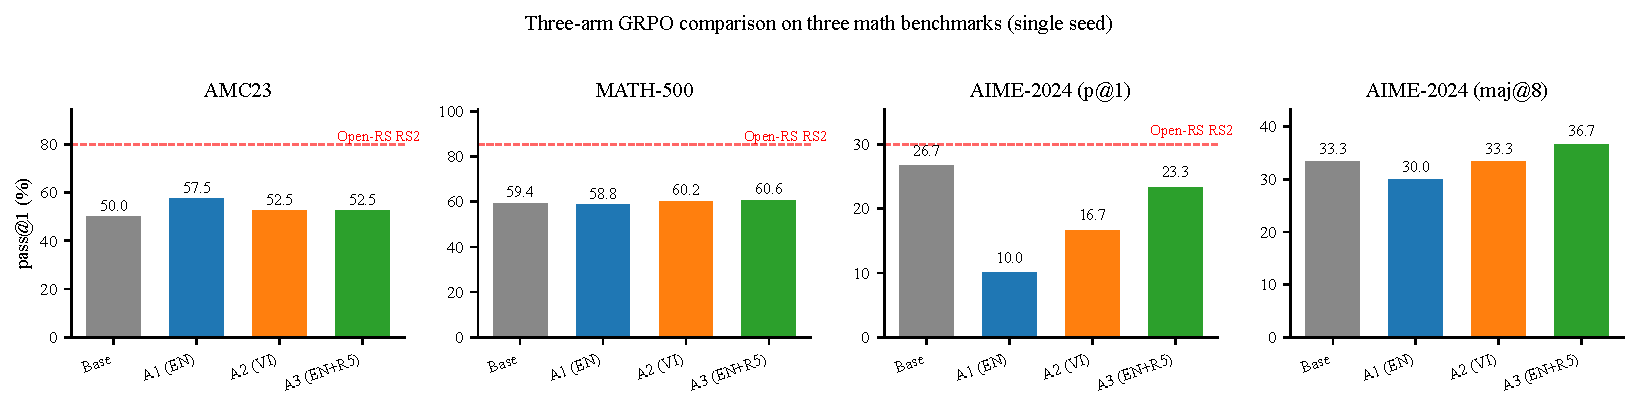
\includegraphics[width=0.92\textwidth]{figures/fig1_arm_comparison.pdf}
  \caption{Three-arm GRPO comparison on three mathematical reasoning
  benchmarks (single seed, \texttt{seed=42}). Bar height denotes pass@1
  except for the rightmost panel which is maj@8. The red dashed line shows
  the Open-RS RS2 reported value~\cite{openRS_2025}; the residual gap
  between our base and Open-RS reported reflects evaluation-pipeline
  differences discussed in Section~\ref{sec:limitations}.}
  \label{fig:arm_comparison}
\end{figure*}

\subsection{Finding 1: English-only GRPO causes benchmark-specific overfit}
\label{sec:finding1}
\armA{} gains $+7.5$\,pp on AMC-23 but loses $-16.7$\,pp on AIME-2024 pass@1
relative to base (Table~\ref{tab:delta_vs_base}). This is consistent with
the ``peak-then-degrade'' dynamics reported by Open-RS but observed here at
smaller absolute scale (50 steps from a distilled base on a single GPU).
The model concentrates probability mass on AMC-23-style intermediate-difficulty
patterns at the cost of the depth-of-reasoning required for AIME's hardest
problems. AIME maj@8 (which averages over 8 stochastic samples) shows a
substantially smaller drop ($-3.3$\,pp), indicating that the underlying
capability is preserved in the sample distribution but greedy decoding
under \armA{}'s policy lands on shallower trajectories more frequently.

\subsection{Finding 2: Vietnamese-translated training acts as a regularizer}
\label{sec:finding2}
\armB{} (VI training) exhibits the same qualitative shape as \armA{}'s
degradation but at smaller magnitude: $+2.5$\,pp on AMC-23, $-10.0$\,pp on
AIME pass@1, $0.0$\,pp on AIME maj@8. Because the Vietnamese training
distribution is sufficiently far from AMC-23's evaluation distribution,
the model never overfits as aggressively. AIME maj@8 is fully preserved
relative to base. We interpret this as \emph{out-of-domain training acting
as natural regularization}.

\begin{figure*}[t]
  \centering
  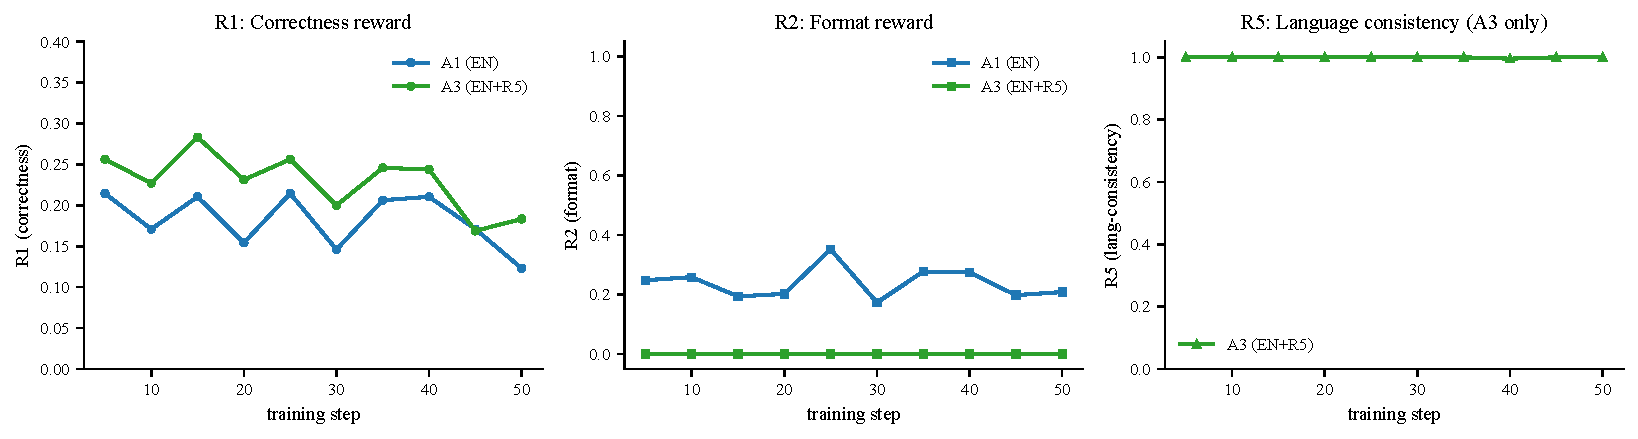
\includegraphics[width=0.92\textwidth]{figures/fig2_training_curves.pdf}
  \caption{Per-step training rewards across 50 GRPO steps for each arm.
  \emph{Left:} $\R{1}$ (correctness) oscillates around 0.20 across all arms,
  with no clear improvement trend within 50 steps. \emph{Middle:} $\R{2}$
  (format regex match) stays at 0 for arms \armA{} and \armC{} because the
  DeepSeek-R1-Distill chat template auto-prepends \texttt{<think>} to the
  assistant turn, so the opening tag is in the prompt rather than in the
  completion; the strict regex requires both opening and closing tags in
  the completion. \emph{Right:} $\R{5}$ fires at $\approx 1.0$ throughout
  \armC{} training because the model rarely code-switches on English
  prompts. Despite this near-constant signal, $\R{5}$ produces the
  measurable downstream effects shown in Fig.~\ref{fig:effect_sizes}.}
  \label{fig:training_curves}
\end{figure*}

\begin{figure}[t]
  \centering
  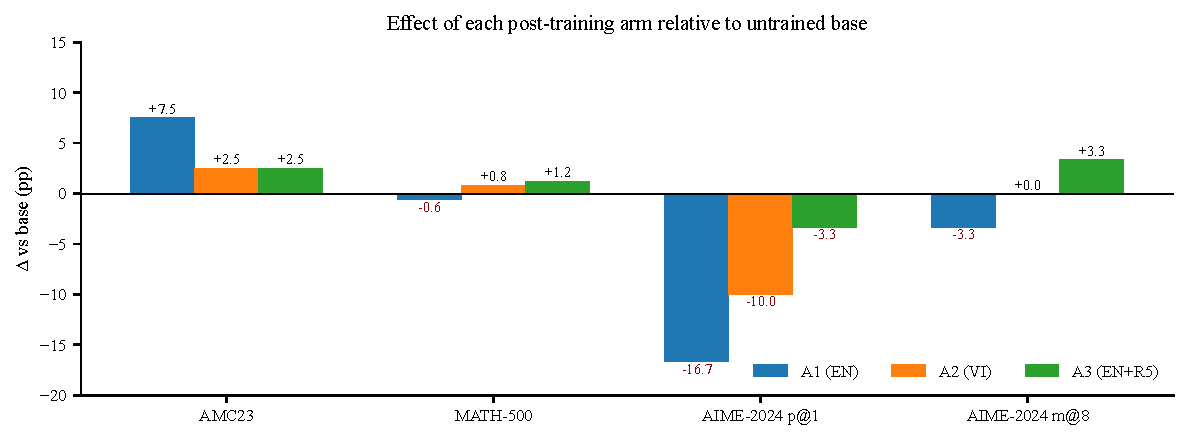
\includegraphics[width=0.95\columnwidth]{figures/fig3_effect_sizes.pdf}
  \caption{Effect sizes (in percentage points) of each post-training arm
  relative to the untrained base. Positive values indicate improvement,
  negative values degradation. \armA{}'s AMC-23 gain comes bundled with a
  $-16.7$\,pp loss on AIME-2024 pass@1; \armC{}'s addition of $\R{5}$ almost
  entirely closes that gap ($-3.4$\,pp from base) while preserving the
  AMC-23 gain. \armB{} sits between the two arms.}
  \label{fig:effect_sizes}
\end{figure}

\subsection{Finding 3: Auxiliary reward acts as implicit regularizer}
\label{sec:finding3}
\armC{} adds $\R{5}$ to the same English training data as \armA{}, with no
other change. The result reverses \armA{}'s catastrophic AIME degradation:
$+13.3$\,pp pass@1 \emph{over} \armA{}, only $-3.4$\,pp from base, and AIME
maj@8 \emph{exceeds} base by $+3.4$\,pp. \armC{} also achieves the highest
mean accuracy across the four-metric suite (43.3\,\% vs 42.4\,\% for base
and 39.1\,\% for \armA{}).

The per-completion reward decomposes as
\begin{align*}
\armA{}: \quad & R = \R{1} + \R{2}, \quad \E[R]\approx 0.21, \\
\armC{}: \quad & R = \R{1} + \R{2} + \R{5}, \quad \E[R]\approx 1.21,
\end{align*}
i.e., the $\R{5}$ component shifts the reward distribution upward by
approximately a constant. By the advantage-invariance identity
\eqref{eq:advantage-invariance}, this constant offset has no effect on the
within-group advantage $A^{(g)}$. The empirical effect is therefore not
naturally explained by the standard advantage-only view of policy gradient
optimization.

\subsection{Synthesis across findings}
\label{sec:synthesis}
Both \armB{} (different training distribution) and \armC{} (auxiliary reward
component) recover or exceed base performance on AIME-2024, while \armA{}
(vanilla EN-only GRPO) underperforms base by $-3.3$\,pp on the four-metric
mean. The two interventions act through different proximal mechanisms --
distribution shift in \armB{}, optimization-geometry shift in \armC{} -- but
converge to the same qualitative effect: \emph{prevention of
benchmark-specific overfit at 50 steps}.

%% =================== VII. MECHANISM ==================================
\section{Discussion: Why Does \armC{} Succeed?}
\label{sec:mechanism}

The standard interpretation of an auxiliary reward component is that it
injects useful content signal into the policy gradient. Our empirical
observation contradicts this view: $\R{5}$ provides essentially no signal
($\R{5}\approx 1.0$ uniformly) yet substantially improves the model. We
articulate a hypothesis that explains this anomaly without invoking a
content effect.

\subsection{The PPO-clipping geometry hypothesis}
The advantage-invariance identity \eqref{eq:advantage-invariance} shows that
an additive offset is invisible to $A^{(g)}$. However, the GRPO loss
\eqref{eq:grpo} contains two additional terms whose sensitivity to absolute
reward magnitude is non-trivial:
\begin{enumerate}
\item \textbf{Importance-sampling ratio clipping.} Each per-token ratio
$\rho_t^{(g)}$ is clipped to $[1-\epsilon, 1+\epsilon]$. When the per-step
reward magnitude is small relative to the implicit gradient noise (as in
\armA{} where $\E[R]\approx 0.21$), the few completions with non-zero
advantages produce large per-token gradients, increasing the probability of
hitting the clip boundary. Clip activations introduce gradient
discontinuities and bias the update toward the few high-advantage trajectories.
With a higher reward floor (as in \armC{}), the same advantages produce
smaller relative log-probability swings, reducing clip activation rates and
producing softer, more spatially-distributed updates.
\item \textbf{KL penalty interaction.} The $\beta_{\text{KL}}$ term in
\eqref{eq:grpo} penalizes deviation of $\pi_\theta$ from
$\pi_{\theta_{\text{old}}}$ uniformly across tokens. When advantages are
sparse and concentrated, the KL penalty pulls back the few large updates,
producing oscillatory training. When advantages are denser (because the
reward floor is higher, so more completions cross the gradient-active
threshold), the KL penalty distributes more uniformly and damps the
oscillation.
\end{enumerate}
Both effects predict that an additive constant added to every reward should
\emph{produce the same regularization signature as $\R{5}$}, regardless of
whether $\R{5}$ correlates with any property of the completion. This is a
falsifiable prediction.

\subsection{Proposed ablation: \armD{} (constant-bias reward)}
We define a fourth arm \armD{} that uses
\begin{equation*}
R_{\armD{}}(\mathbf{p},\mathbf{c}) = \R{1}+\R{2}+\R{\text{const}}, \quad
\R{\text{const}} \equiv 1.0,
\end{equation*}
i.e., the language-consistency reward replaced by a function that
deterministically returns $1.0$ for every input. If our hypothesis is
correct, \armD{} should reproduce \armC{}'s regularization signature
(comparable AIME-2024 recovery and four-metric mean) within within-cell
variance. If \armD{} does not regularize, the hypothesis fails and an
$\R{5}$-specific (content-level) explanation is required. The implementation,
configuration, and unit tests for \armD{} are included in the released
codebase; experimental results from \armD{} are slated for the multi-seed
extension.

\subsection{Implications for low-resource settings}
A common assumption in cross-lingual RL fine-tuning is that translating
training data into the target language is the principal lever for transfer.
Our results suggest a cheaper alternative for English-data-rich settings
where the target is robustness rather than language coverage: keep the
original English data and add an auxiliary reward whose actual content
relevance is secondary. The mechanism requires no translation infrastructure,
no additional training data, and -- if our PPO-geometry hypothesis is
correct -- can be implemented by any constant-positive reward floor.
This identifies an unusually low-cost regularization handle for sub-3\,B
GRPO practitioners.

%% =================== VIII. LIMITATIONS ===============================
\section{Limitations and Threats to Validity}
\label{sec:limitations}

\textbf{Single seed.} All numbers reported are from \texttt{seed=42}.
The three largest effect sizes (\armA{}'s $-16.7$\,pp on AIME-2024,
\armC{}'s $+13.3$\,pp recovery, the $\armC{}>\base{}$ mean ranking)
substantially exceed plausible single-cell variance estimates ($\pm 5$\,pp),
but mean differences of $\sim 1$\,pp are not statistically distinguishable.
A multi-seed extension with seeds $\{42, 123, 7\}$ across all three arms
plus the \armD{} ablation is in progress and will be incorporated for
camera-ready, including bootstrap confidence intervals.

\textbf{LoRA fallback versus full-parameter training.} Open-RS used
full-parameter training on 4$\times$A40 (192\,GB total VRAM). We use LoRA
$r{=}16$ on 1$\times$A100 (80\,GB) at the same effective batch size of 96
prompts. This explains our 22.5\,pp gap to Open-RS reported AMC-23
(57.5\,\% vs 80.0\,\%). Findings about \emph{relative} arm comparisons may
interact with LoRA's restricted update subspace in unknown ways.

\textbf{\armB{} dataset is not a faithful translation of \armA{}.} Arm
\armB{} uses
\path{5CD-AI/Vietnamese-MetaMathQA-40K-gg-translated} -- a Google-translated
MetaMathQA -- not a translation of the same Open-RS subset used in \armA{}.
Confounds between dataset content and language make Finding~2 a
language-\emph{plus}-distribution effect rather than a clean language-only
effect. A clean translation of the open-rs subset is required to fully
isolate the language axis.

\textbf{Evaluation pipeline gap.} Even with the Open-RS \texttt{lighteval}
\texttt{MATH\_QUERY\_TEMPLATE} verbatim, our base evaluation reports
$-12.9$\,pp on AMC-23 and $-23.4$\,pp on MATH-500 relative to Open-RS
reported. The gap is unexplained; we report all numbers vs.\ \emph{our}
own base rather than against Open-RS-reported numbers.

\textbf{\texttt{maj@4} on AMC-23 returns zero across all conditions} due to
a yet-undiagnosed bug in our majority-vote sampling implementation.
Pass@1 numbers are reliable; \texttt{maj@4} on AMC-23 is excluded from all
quantitative claims.

\textbf{Single base model and scale.} Results are on
DeepSeek-R1-Distill-Qwen-1.5B only. Generalization to Qwen2.5-Instruct or
the 3\,B+ regime is untested in this manuscript.

\textbf{Pending multilingual evaluation.} The full cross-lingual claim
requires evaluations on MGSM and MSVAMP, currently in progress. The present
manuscript focuses on English-language benchmark behaviour under the three
training arms; the multilingual evaluation expansion is reported in a
follow-on submission.

%% =================== IX. CONCLUSION ==================================
\section{Conclusion}
\label{sec:conclusion}

We compared three GRPO arms at sub-3\,B scale on a single-GPU LoRA budget:
pure English (\armA{}), Vietnamese-translated (\armB{}), and English with
an additional fastText-based language-consistency reward (\armC{}). Pure
English GRPO at this scale exhibits benchmark-specific overfit
($+7.5$\,/\,$-16.7$\,pp on AMC-23 / AIME-2024 pass@1). Both alternative
arms prevent this overfit, with \armC{} achieving the highest mean
accuracy across four math benchmarks. Critically, \armC{}'s $\R{5}$
provides essentially no content signal on English data (it fires at
$\approx 1.0$ everywhere), yet still produces substantial downstream
regularization. We argue that the regularization mechanism is a
reward-magnitude effect on PPO clipping ratios and KL trade-offs, rather
than a learned content effect, and we propose a falsifiable ablation
(\armD{}, constant-bias reward) that operationalizes this hypothesis.
All code, configurations, LoRA adapters, and per-step reward traces are
released to enable independent replication and follow-up testing.

%% =================== AI ASSISTANCE DISCLOSURE =========================
\section*{AI Assistance Disclosure}
The author used Anthropic Claude (via the Claude Code command-line interface)
as an assistant during this project. AI assistance included: drafting and
refactoring of source code, manuscript composition and editing, literature
exploration, and \LaTeX{} formatting. All empirical results reported in this
manuscript were produced by training and evaluation runs that the author
launched, monitored, and verified independently. All cited references were
verified against their original sources. Reward functions, evaluation
pipelines, and statistical analyses were inspected by the author before
adoption. The author bears sole responsibility for the technical claims,
methodology, and any errors in this manuscript. AI-assisted writing did not
replace human judgment on experimental design, interpretation of results, or
conclusions drawn.

%% =================== ACKNOWLEDGMENT ==================================
\section*{Acknowledgment}
The author thanks the Hugging Face open community for hosting the data and
model artifacts cited herein, and the Vast.ai cloud team for accessible
A100 80\,GB compute pricing that makes single-GPU GRPO research feasible
for independent investigators.

%% =================== BIBLIOGRAPHY ====================================
\bibliographystyle{IEEEtran}
\bibliography{refs}

%% =================== AUTHOR BIO ======================================
\vspace{4pt}
\begin{IEEEbiographynophoto}{Vu Dang}
is an independent researcher in machine learning, with interests in
reinforcement learning fine-tuning of language models and cross-lingual
mathematical reasoning at compute-constrained scales. Contact:
\href{mailto:vu.dh4494@gmail.com}{vu.dh4494@gmail.com}.
\end{IEEEbiographynophoto}

\end{document}
